% DO NOT COMPILE THIS FILE DIRECTLY!
% This is included by the other .tex files.
\section*{Estimadores bayesianos}
\begin{frame}{Estatística bayesiana}
 \begin{itemize}
  \item Os paradigmas bayesiano e frequentista; 
  \item Distribuição~\textit{a priori} e~\textit{a posteriori};
%   \item Sensibilidade e prioris impróprias;
  \item Função de verossimilhança;
  \end{itemize}  
  \begin{columns}
    \begin{column}{0.5\textwidth}
        \begin{figure}[!ht]
        \label{fig:bayes_sign}
        \begin{center}
        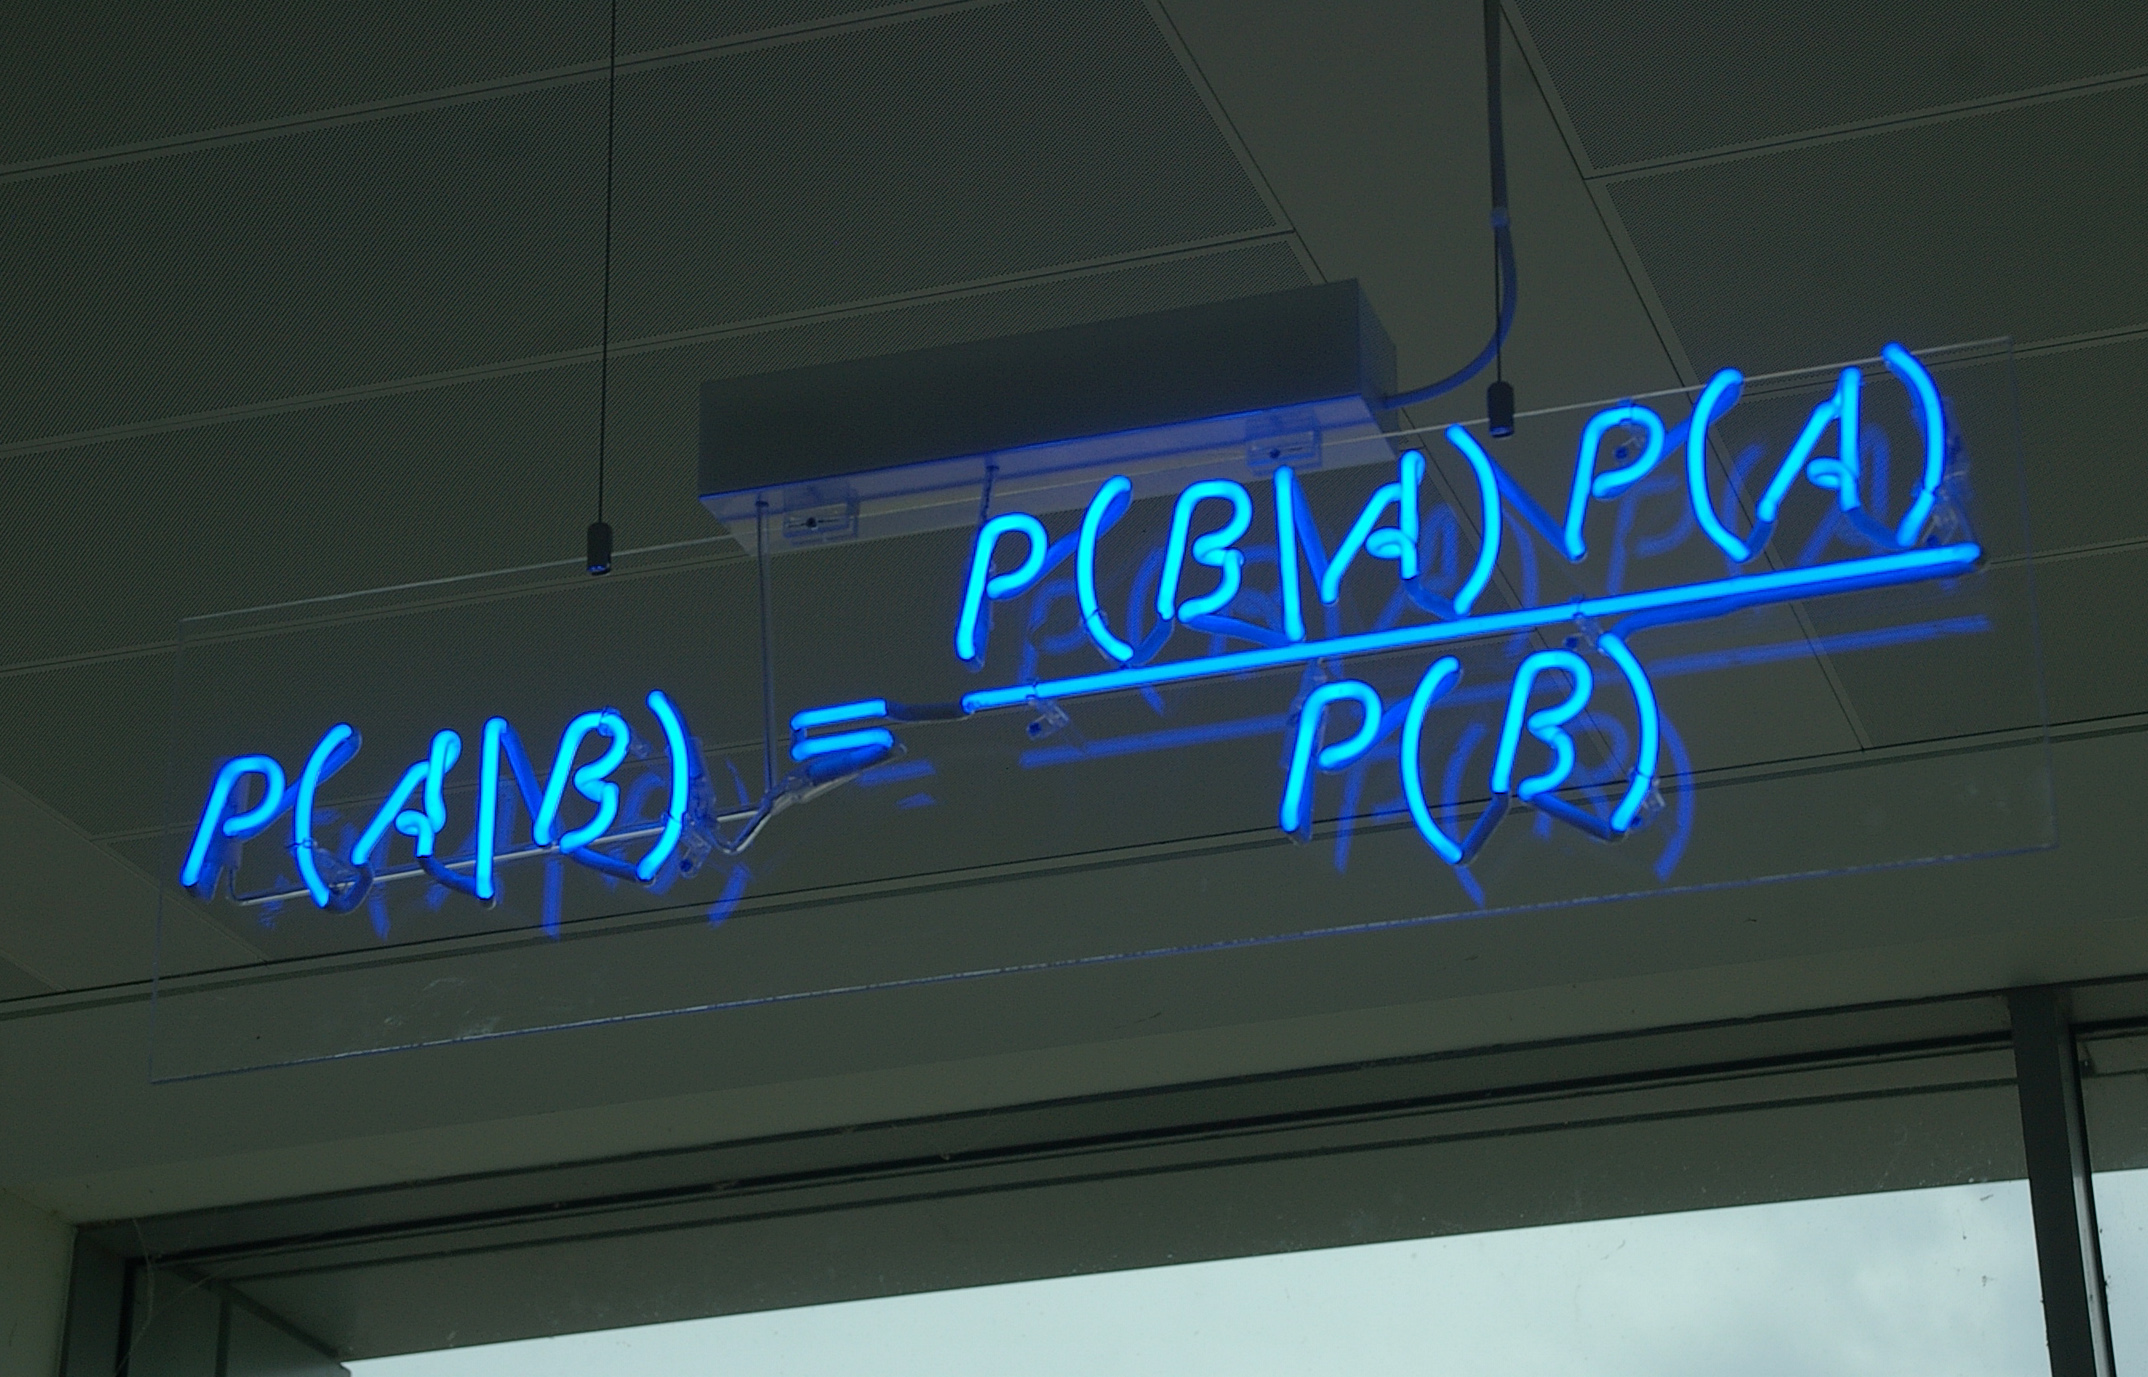
\includegraphics[scale=0.07]{figures/Bayes_Theorem_MMB_01.jpg} 
        \end{center}
        \end{figure}        
    \end{column}
\begin{column}{0.5\textwidth}
   \begin{figure}[!ht]
    \label{fig:bayes_graph}
    \begin{center}
    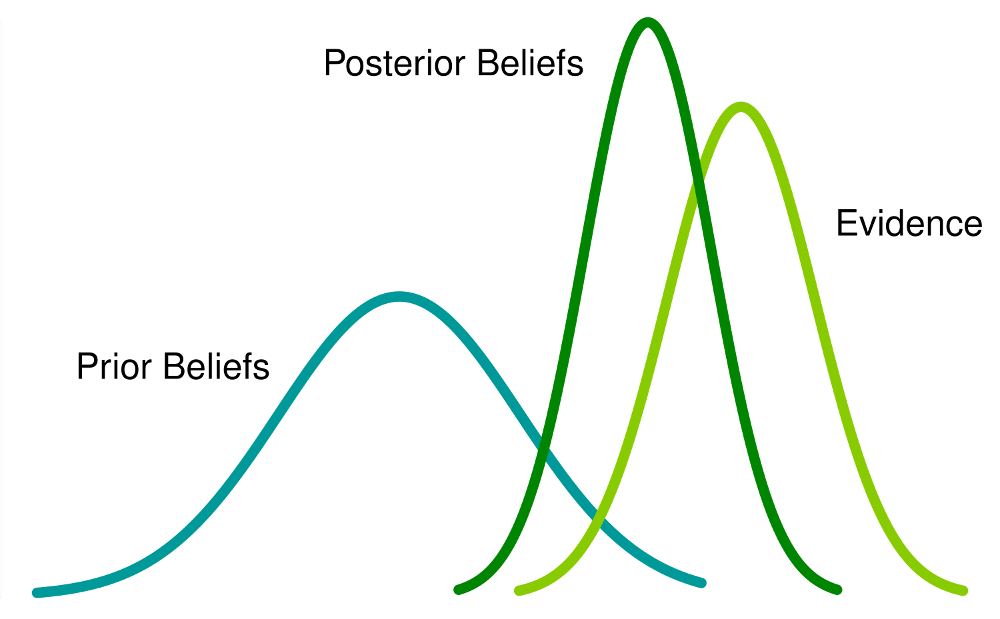
\includegraphics[scale=1.0]{figures/bayesian_inference.jpg} 
    \end{center} 
    \end{figure} 
\end{column}
  \end{columns}  
\end{frame}
%%%%%%%%%%%%%%%%%%%%%%%%%%%%%%%%%%%
\begin{frame}{Permutabilidade}
\begin{defn}[Permutabilidade]
\label{def:exchangeability}
 \textbf{Permutabilidade}.
 Uma coleção finita de variáveis aleatórias $\rs$ com densidade conjunta $f$ é dita~\textbf{permutável} se 
 \[f(x_1, x_2, \ldots, x_n) = f( x_{\pi(1)}, x_{\pi(2)}, \ldots, x_{\pi(n)} ), \]
 para qualquer permutação $\boldsymbol\pi = \{\pi(1), \pi(2), \ldots, \pi(n)\}$ dos seus elementos.
 Uma coleção infinita é permutável se qualquer subconjunto finito é permutável.
\end{defn}
\begin{itemize}
 \item Note que uma amostra permutável não precisa ser independente;
 \item Note também que IID $\implies$ permutável;
 \item A intuição é simples: simetria.
\end{itemize}
\end{frame}
%%%%%%%%%%%%%%%%%%%%%%%%%%%%%%%%%%%
\begin{frame}{Parâmetros como limites de variáveis aleatórias.}
\begin{exemplo}
\label{ex:remission}
 \textbf{Ensaio Clínico (DeGroot, exemplo 7.1.3).}
 Suponha que estamos interessados na taxa de recrudescência (``recaída'') de uma determinada doença entre pacientes tratados com uma droga.
 Seja $X_i$ a variável aleatória que indica se o $i$-ésimo paciente recrudesceu ($X_i = 1$) ou não ($X_i = 0$).
 Seja $P$ a proporção de indivíduos que recrudescem num grupo grande de pacientes. 
 Se $P$ é desconhecida, podemos modelar $\irs$ como variáveis aleatórias Bernoulli IID com parâmetro $p$~\textbf{condicional} a $P = p$.
 Em notação estatística:
 \[ \irs \mid P = p \sim \operatorname{Bernoulli}(p).\]
  \textbf{Assuma} que $\irs$ é uma sequência permutável infinita.
  Agora chamemos de $P_n$ a proporção de pacientes que recrudescem nos $n$ primeiros pacientes.
  Podemos mostrar que o limite $\lim_{n \to \infty} P_n = \lim_{n \to \infty} \sum_{i=1}^n X_i/n$ existe com probabilidade 1 e que pode ser visto como a proporção $P$.
\end{exemplo}
\end{frame}
%%%%%%%%%%%%%%%%%%%%%%%%%%%%%%%%%%%
\begin{frame}{Paradigmas de inferência}
No Exemplo~\ref{ex:remission} podemos encarar o problema de duas maneiras:
\begin{itemize}
 \item[A)] $P$ é uma variável aleatória e $\irs$ são $\operatorname{Bernoulli}(p)$~\textbf{condicional} ao evento $P = p$, $p \in (0, 1)$.
 \item[B)] Para uma constante fixa (e inobservável) $p$, $\irs$ tem distribuição $\operatorname{Bernoulli}$ com parâmetro $p$ -- isto é, indexada por $p \in (0, 1)$.
\end{itemize}
Uma diferença~\textit{sutil}, não é?
A tradição estatística que entende parâmetros como variáveis aleatórias como em A) é chamada de \textbf{Estatística bayesiana}\footnote{Em homenagem ao reverendo inglês Thomas Bayes (1701 -- 1761).}.
Já os que aderem à abordagem B) são chamados~\textbf{frequentistas} -- ou ortodoxos, como Jaynes gosta de chamá-los.
Neste curso veremos conceitos e exemplos destas duas escolas de pensamento. 
\end{frame}
%%%%%%%%%%%%%%%%%%%%%%%%%%%%%%%%%%%
\begin{frame}{Uma análise bayesiana}
\begin{exemplo}[Duração de componentes]
\label{ex:duracao_componentes}
\textbf{Duração de componentes eletrônicos (DeGroot, exemplo 7.2.1).}
Suponha que uma empresa esteja interessadas em saber o quanto duram os produtos que ela produz.
Se representamos os tempos de duração de $n$ objetos como $n$ variáveis aleatórias $\rs$ IID com distribuição exponencial com parâmetro $\theta$ de modo que
$$f(x_i \mid \theta) = \theta \exp(-\theta x_i), x_i > 0.$$
\textbf{Observação:} $n/\sum_{i=1}^n X_i \xrightarrow{\text{p}} \theta$.

Aqui, $\theta$ é a taxa de falha dos componentes, e é um parâmetro de interesse.
Suponha que uma pessoa experiente na empresa diga que a taxa de falha é mais ou menos $0.5$/ano.
Como representamos esta informação?
\end{exemplo} 
\end{frame}
%%%%%%%%%%%%%%%%%%%%%%%%%%%%%%%%%%%
\begin{frame}{Uma análise bayesiana (cont.)}
 \begin{figure}[!ht]
\label{fig:gamma_1_2}
\begin{center}
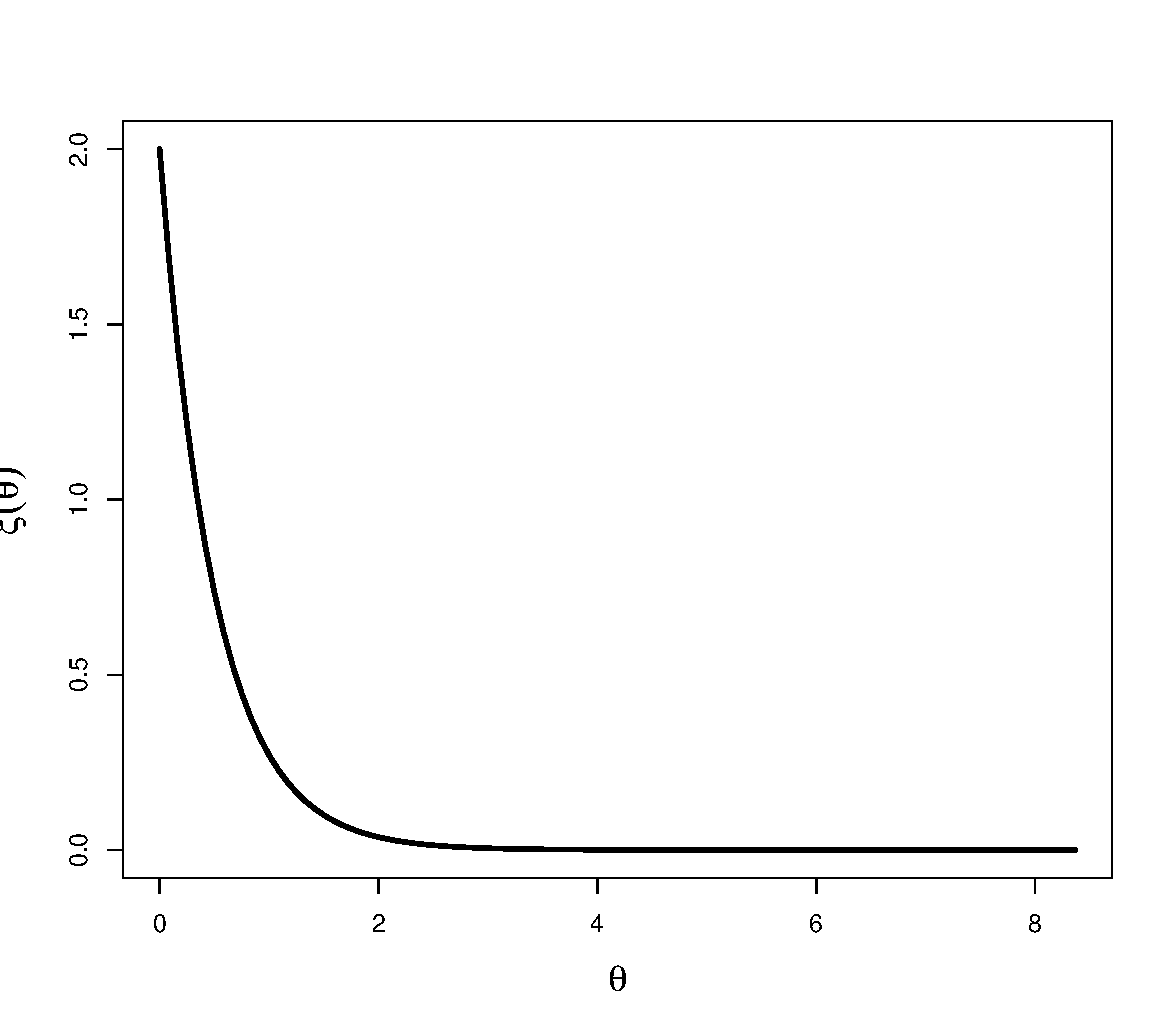
\includegraphics[scale=0.4]{figures/gamma_1_2.pdf} 
\end{center} 
\end{figure} 
\end{frame}
%%%%%%%%%%%%%%%%%%%%%%%%%%%%%%%%%%%
\begin{frame}{A distribuição~\textit{a priori}}
\begin{defn}[Distribuição~\textit{a priori}]
\label{def:prior}
 Se tratamos o parâmetro $\theta$ como uma variável aleatória, então a distribuição~\textit{a priori}, que também chamaremos simplesmente de priori, é a distribuição que damos a $\theta$~\textbf{antes} de observarmos as outras variáveis aleatórias de interesse.
 Em geral, vamos denotar a função de densidade/massa de probabilidade da priori por $\xi(\theta)$.
\end{defn}
\textbf{Exemplos:}
\begin{itemize}
 \item Podemos dizer que a probabilidade de uma moeda cair cara, $p$, tem distribuição uniforme entre 0 e 1;
 \begin{itemize}
  \item Ou que tem distribuição $\operatorname{Beta}(2, 2)$;
 \end{itemize}
 \item A altura média dos jogadores de basquete do CR Flamengo tem distribuição normal com média $\mu_0 = 200 cm$ e variância $\sigma_0^2 = 25 cm^2$;
 \item A posição de Júpter em relação ao Sol hoje tem coordenadas $X,Y, Z$, de modo que $X \sim \operatorname{Normal}(\mu_x, 1)$, $Y \sim \operatorname{Normal}(\mu_y, 1)$, $Z \sim \operatorname{Normal}(\mu_z, 1)$.
\end{itemize}
\end{frame}
%%%%%%%%%%%%%%%%%%%%%%%%%%%%%%%%%%%
\begin{frame}{Distribuição~\textit{a posteriori}}
\begin{defn}[Distribuição~\textit{a posteriori}]
 \label{def:posterior}
 Considere o problema estatístico com parâmetro $\theta$ e variáveis aleatórias observáveis $\rs$.
 A distribuição condicional de $\theta$ dados os valores observados das variáveis aleatórias, $\boldsymbol x := \{x_1, x_2, \ldots, x_n \}$ é a~\textbf{distribuição~\textit{a posteriori}} de $\theta$.
 Denotamos por $\xi(\theta \mid \boldsymbol x)$ a f.d.p/f.m.p. condicional a $X_1 = x_1, X_2 = x_2, \ldots X_n = x_n$.
\end{defn}
\begin{theo}[Distribuição~\textit{a posteriori}: derivação]
 \label{thm:posterior_distribution}
 Considere a amostra aleatória $\rs$ de uma distribuição com f.d.p./f.m.p. $f(x\mid\theta)$.
 Se a distribuição~\textit{a priori} é $\xi(\theta)$, temos
 \begin{equation}
  \label{eq:posterior}
    \xi(\theta \mid \boldsymbol x) = \frac{\xi(\theta)\prod_{i=1}^n f(x_i \mid \theta)}{g_n(\boldsymbol x)}, \: \theta \in \Omega.  
 \end{equation}
 Chamamos $g_n(\boldsymbol x)$ de distribuição~\textit{marginal} de $\rs$.
\end{theo}
\textbf{Prova:} Usar a premissa de amostra aleatória para escrever $f(x_1, x_2, \ldots, x_n \mid \theta)$, escrever a distribuição conjunta de $\theta$ e $\boldsymbol x$ e computar $g_n(\boldsymbol x)$ usando a lei da probabilidade total. 
\end{frame}
%%%%%%%%%%%%%%%%%%%%%%%%%%%%%%%%%%%
\begin{frame}{Distribuição~\textit{a posteriori}: exemplo}
Continuando com o Exemplo~\ref{ex:duracao_componentes}, fica claro que 
 \[f (\boldsymbol x  \mid \theta) = \prod_{i=1}^n f(x_i \mid \theta) = \theta^n\exp(-S\theta), \]
onde $S = \sum_{i = 1}^n x_n$.
Desta forma, temos 
\[ f (\boldsymbol x  \mid \theta)\xi(\theta) = \theta^{n}\exp(-(S + 2)\theta).\]
Para obter $g_n(\boldsymbol{x})$, computamos 
\[ g_n(\boldsymbol{x}) = \int_0^\infty t^{n}\exp(-(S + 2)t) \,dt = \frac{\Gamma( n + 1) }{ (S + 2)^{n + 1}}. \]
Concluímos que 
\[\xi(\theta \mid \boldsymbol{x}) = \frac{(S + 2)^{n + 1}}{\Gamma( n + 2)} \theta^{n+1}\exp(-(S + 2)\theta),  \]
ou seja, $\theta \mid \boldsymbol{x} \sim \operatorname{Gama}(n + 1, \sum_{i = 1}^n x_n + 2)$.
\end{frame}
%%%%%%%%%%%%%%%%%%%%%%%%%%%%%%%%%%%
\begin{frame}{Distribuição~\textit{a posteriori}: exemplo (cont.)}
    \begin{figure}[!ht]
    \label{fig:posterior_componentes}
    \begin{center}
    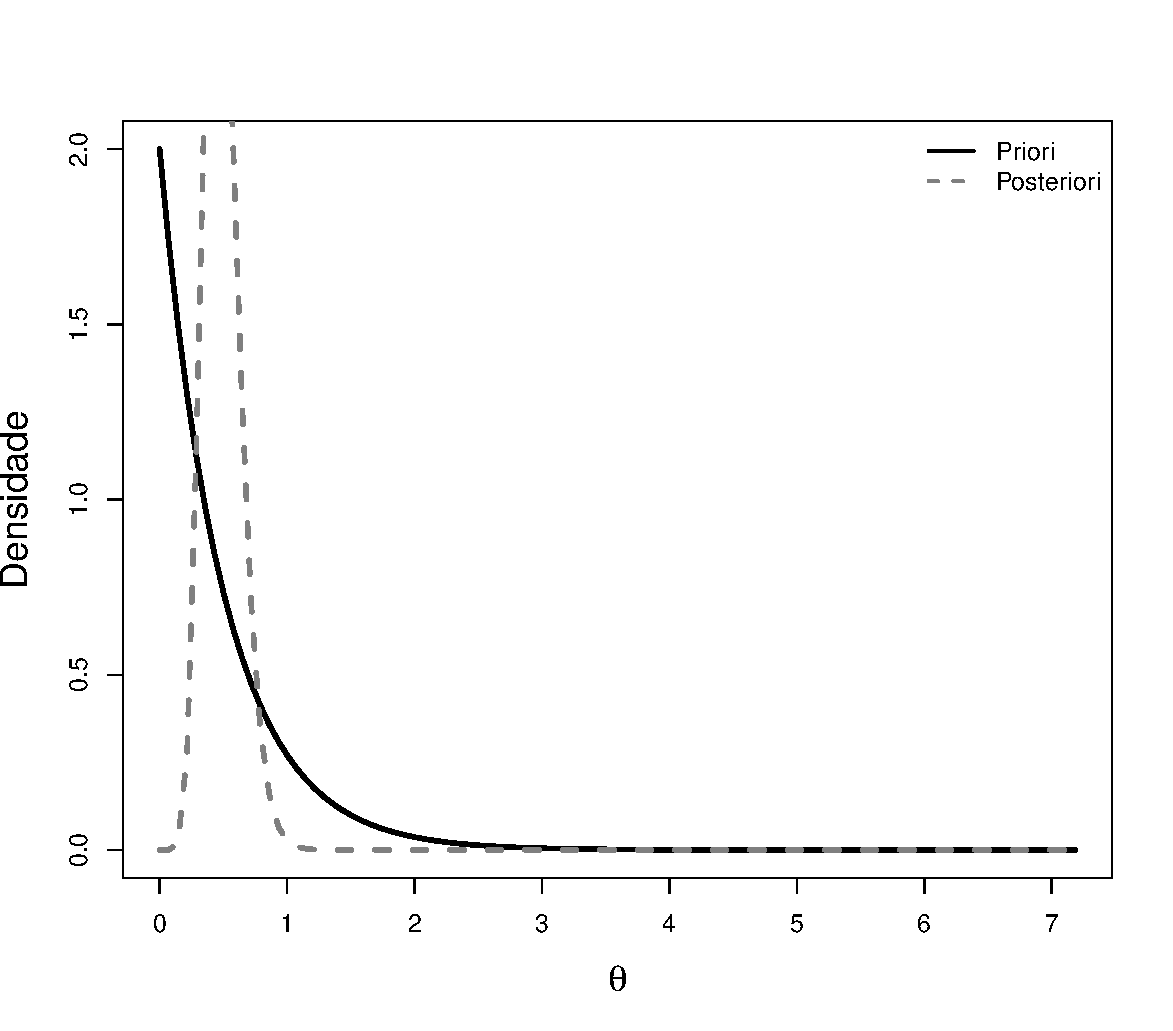
\includegraphics[scale=0.4]{figures/posterior_componentes.pdf} 
    \end{center} 
    \end{figure} 
\end{frame}
%%%%%%%%%%%%%%%%%%%%%%%%%%%%%%%%%%%
\begin{frame}{A função de verossimilhança}
 Note que o denominador em~(\ref{eq:posterior}) não depende do parâmetro, $\theta$.
 Deste modo, podemos escrever
 \[ \xi(\theta \mid \boldsymbol{x}) \propto f(\boldsymbol{x} \mid \theta)\xi(\theta), \]
 querendo dizer que os dois lados de $\propto$ são iguais a não ser talvez por uma constante que independe de $\theta$.
 Por vezes podemos escrever também $\xi(\theta \mid \boldsymbol{x}) \propto_\theta f(\boldsymbol{x} \mid \theta)\xi(\theta)$.
 \begin{defn}[Função de verossimilhança]
 \label{def:likelihood_function}
  Quando encaramos a f.d.p./f.m.p. $f(x_1, x_2, \ldots, x_n \mid \theta)$ como uma função do parâmetro $\theta$, chamamos esta função de~\textbf{função de verossimilhança}, e podemos denotá-la como $L(\theta ; \boldsymbol{x})$ ou, quando a notação não criar ambiguidade, simplesmente $L(\theta)$.
 \end{defn}
\end{frame}
%%%%%%%%%%%%%%%%%%%%%%%%%%%%%%%%%%%
\begin{frame}{Aprendizado bayesiano sequencial}
Ainda sobre o Exemplo~\ref{ex:duracao_componentes}, considere a primeira observação $x_1$ e a distribuição~\textit{a posteriori} baseada apenas nesta observação: $\xi_1(\theta \mid x_1) \propto f(x_1 \mid \theta)\xi(\theta)$.
Se assumirmos que $\rs$ são condicionalmente independentes dado $\theta$, podemos escrever 
\[\xi(\theta \mid x_1, x_2) \propto f(x_1, x_2 \mid \theta)\xi(\theta) = f(x_1 \mid \theta)f(x_2 \mid \theta)\xi(\theta) = f(x_2 \mid \theta)\xi_1(\theta \mid x_1). \]
    \begin{figure}[!ht]
    \label{fig:posterior_componentes_sequencial}
    \begin{center}
    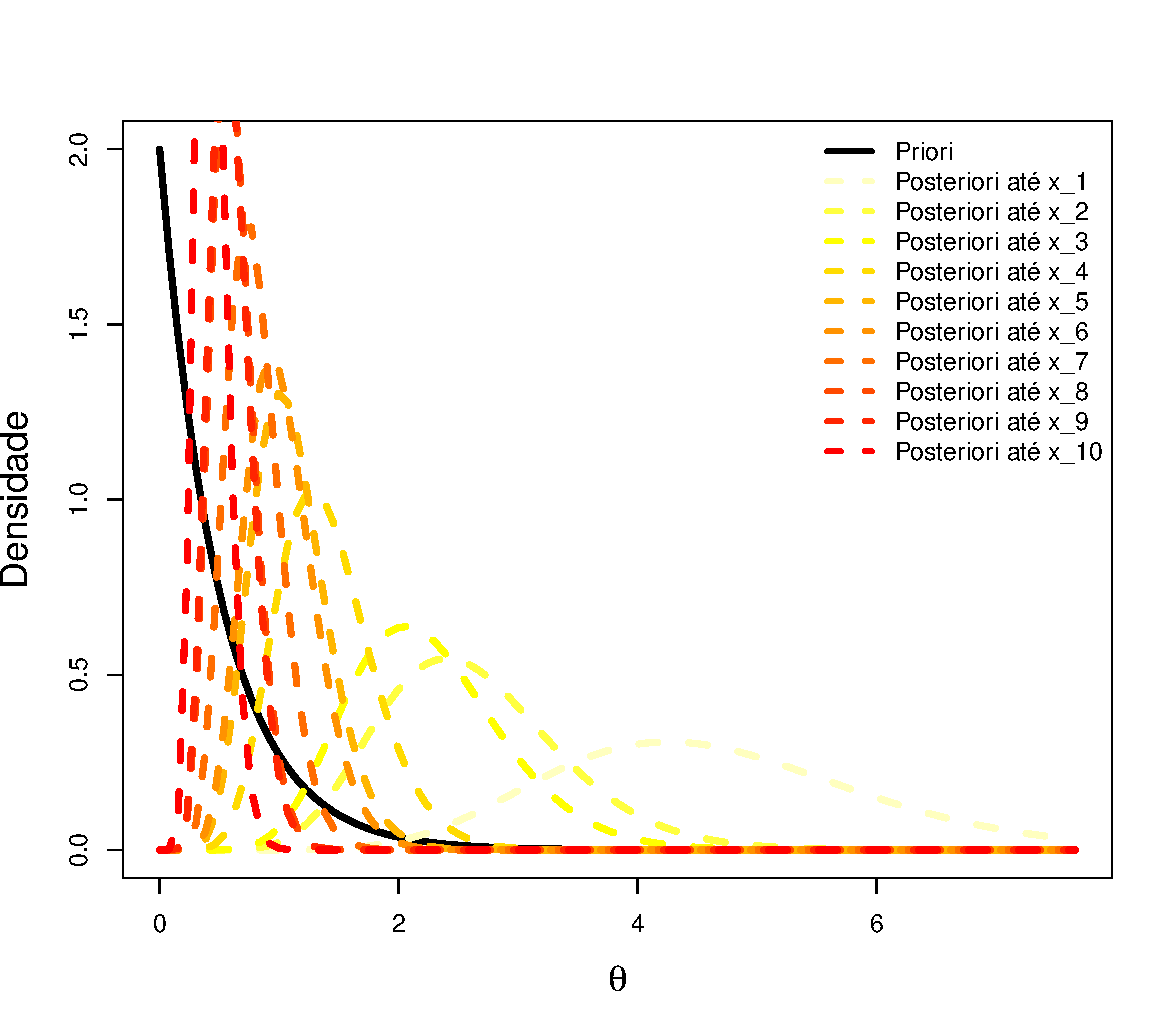
\includegraphics[scale=0.32]{figures/sequential_Bayes_componentes.pdf} 
    \end{center} 
    \end{figure} 
\end{frame}
%%%%%%%%%%%%%%%%%%%%%%%%%%%%%%%%%%%
\begin{frame}{Predição}
 Dentro do paradigma bayesiano, a predição de novos valores da(s) variável(is) aleatória(s) é feita a partir da distribuição~\textit{a posteriori},
 \begin{equation}
  \label{eq:posterior_prediction}
  p(X_{n+1} = x_{n+1} \mid x_1, x_2, \ldots, x_n) = \int_{\Omega} f(x_{n+1} \mid \theta)\xi(\theta \mid x_1, x_2, \ldots, x_n)\, d\theta.
 \end{equation}
Chamamos a distribuição condicional em~(\ref{eq:posterior_prediction}) de~\textbf{distribuição preditiva~\textit{a posteriori}}.
Em contraste, temos a~\textbf{distribuição preditiva~\textit{a priori}}:
 \begin{equation}
  \label{eq:prior_prediction}
  p(x_{n+1}) = \int_{\Omega} f(x_{n+1} \mid \theta)\xi(\theta)\, d\theta,
 \end{equation}
que é útil na aplicação de modelos bayesianos na prática, mas não será explorada aqui.
\end{frame}

%%%%%%%%%%%%%%%%%%%%%%%%%%%%%%%%%%%
\begin{frame}{O que aprendemos?}
\begin{itemize}
 \item[\faLightbulbO] Bayesianismo X frequentismo;
 
 ``Parâmetros como variáveis aleatórias ou constantes fixas e não-observáveis.''
 
 \item[\faHourglassStart] Distribuição~\textit{a priori}, $\xi(\theta)$;
 
 ``Nosso grau de crença~\underline{antes} de observamos dados.''
 
 \item[\faInfoCircle] Função de verossimilhança, $L(\theta) \propto f(\boldsymbol x \mid \theta)$;

 ``Codifica (toda) a informação sobre o modelo contida nos dados.''
 
 \item[\faHourglassEnd] Distribuição~\textit{a posteriori}, $\xi(\theta \mid \boldsymbol x) \propto L(\theta)\xi(\theta)$;
 
 ``Nossa crença atualizada a partir da informação contida em $L(\theta)$.''
 \end{itemize}
\end{frame}
%%%%%%%%%%%%%%%%%%%%%%%%%%%%%%%%%%%
\begin{frame}{Leitura recomendada}
\begin{itemize}
 \item[\faBook] DeGroot seção 7.2;
 \item[\faBook] $^\ast$ Capítulo 1 de Schervish, M. J. (2012). Theory of statistics. Springer Science \& Business Media.
 \item[\faForward] Próxima aula: DeGroot, seção 7.3;
 \item {\large\textbf{Exercícios recomendados}}
 \begin{itemize}
  \item[\faBookmark] DeGroot, seção 7.2: exercícios 2, 3 e 10. 
 \end{itemize}

%  \item[‡\faGithub] .
\end{itemize} 
\end{frame}
